\section{Les supernovae}

\subsection{le modele theorique}
il existe principalement deux événement pouvant mener a un explosion de supernovæ : 

\begin{itemize}
\item soit l'étoile est a l'origine suffisamment massive (plus de 8Mo) pour s'effondrer a la fin de sa vie.
\item soit l'étoile n'est pas suffisamment massive (elle va donc mourir en naine blanche) mais dispose de suffisamment de matière a proximité (généralement étoiles double ou le compagnon pas en phase géante rouge) pour que sa masse augmente avec le temps.
la matière acretté va faitre passer la masse de cette étoile au dessu de la limite.
\end{itemize}

Les étoiles de plus de 8mo exploses en SN en injectant 1e51 erg dans le milieu\\
Cette injection limite fortement la formation stellaire dans le milieu.\\
modèle sous grille\\


\subsection{Les differentes phases}

\begin{itemize}
\item expansion adiabatique
Dans la phase d'expansion adiatique, l'energie est conservé, le choc est violent et le gas n'a pas le temps de perdre de l'énergie par radiation.
Dans cette phase, l'expension est suffisement rapide pour que la dissipation d'énergie par radiation soit négligeable 
C'est le cas dans le test de Sedov

\item snowplow
Dans la phase snowplow, le choc a suffisemment ralentis pour que le gas commence a rayonner de l'energie, l'energie n'est plus conservée.
Dans ce cas, il se forme un bourelet de compression dans lequel le gas est poussé, comme dans le cas d'un chasse neige. 
Les pertes par radiation deviennent importantes. 
\end{itemize}



\subsection{les superbubles}
Dans les endroits de formation stellaire, les étoiles ne sont pas isolées mais apparaisent ensemble au sein d'un même nuage de gas.
L'effondrement gravitationnel du nuage mêne a créer un génération d'etoile en un cours laps de temps.
Toutes ces étoiles vont mourrir dans un laps de temps rapproché et ainsi, les differentes supernovae vont injectée de l'energy dans le milieu dans un temsp tres rapproché.
Les différentes bulle vont se rencontrer (a la manière des bulles ionizées) en mener a une bulle plus grande appelée superbuble.


\subsection{les considérations d'echelles}
La facon de gerer les supernovae sera donc fonction de léchelle que l'on considere.
Dans des simulations tres detaillées de galaxies, il sera necessaire de resoudre la phase adiabatique d'explosion individuelle.
Dans des simulations cosmologiques de la reionisation, l'interet sera plus porté sur la phase snowplow des superbubbles.


\subsection{ Différentes implémentations existantes}



\subsubsection{Navaro and white}


\subsubsection{Stinson et al}



\subsubsection{dubois et Teyssier}

Utilisation de particule fantômes pour simuler les différentes phase

\subsubsection{Dalla Veccia et Schaye}

Modèle probabiliste, injection d'énergie seulement si l'énergie est suffisante pour générer un mouvement suffisant.


\subsection{Mes Implémentations}


\subsubsection{le model thermique}
Le modèle thermique consiste a injecter l'energie sous forme d'energie interne.
Il existe 2 variables d'etat liées a l'energie interne: la pression et la température.
Modifié l'une de ses 2 variables est equivalent.

Dans l'implementation actuelle, la pression est modifiée en utilisant cette conversion:

\begin{equation}
P^{0+} = P^{0-}  + E_0 * (\gamma-1)
\end{equation}

Ce modèle est connu pour avoir de fortes pertes de d'énergie dans le cas ou le refroidissement est autorisé.


\subsubsection{le model cinetique}


Le modèle cinétique consiste a modifier directement la vitesse du gaz autour de l'explosion dans le but de shunter la conversion de l'énergie interne en mouvement.
Ce type de model a été utilisé pour 

Nous avons fait le choix de limiter le nombre de cellules utilisées a 8 correspondant a 1 oct de la structure AMR d'\emma

\begin{equation}
e_{SN} = E_{SN}/8
\end{equation}

Ensuite cette énergie est utilisé pour changer la vitesse du gaz en utilisant : 
\begin{equation}
    \Delta \overrightarrow{v_{gas}} = \sqrt{\frac{2e_{SN}}{\rho_g.dV}} \overrightarrow{u}
    \label{eq_sn_direct}
\end{equation}


\subsection{Test numérique (Sedov)}

%la dérivation des solutions du test de Sedov se trouve :
%chapitre 17 de Shu the physique of astrophysic Volume 2.\\

Dans le but de tester l'implémentation des différents modèles d'injection d'énergie, je l'es ai soumis au test de Sedov.
Ce test est utilisé pour tester le cas d'une explosion parfaite.
Il consiste a relâcher instantanément une quantité d'énergie $E_0$ dans un milieu homogène d'indice adiabatique $\gamma$, de densité $\rho_0$ et de pression $P_0$ (ou de température $T_0$).
Ce brusque changement dans l'état du système créer une discontinuité que le solveur va devoir gérer.

L'avantage de ce test est qu'il dispose d'une solution analytique.
Sedov a exprimé  en 1959 que le rayon de l'explosion en fonction du temps peux s'exprime : %TODO ref

\begin{equation}
r_{(t)}=\left( \frac{E_0}{\alpha \rho_0 }\right)^{1/5} t^{2/5}
\end{equation}


\subsubsection{Sedov évolution temporelle }


parametre du test :
rho=1
p=1e-5
v=0
gamma=5/3


Ce test consiste a suivre l'onde de choc et a s'assurer que son profil et sa position sont correct dans le temps.
On calcul pour chaque cellule sa distance au centre de l'explosion, puis en utilisant un histogramme sur les rayons, pondéré par la valeur du champ que l'on veux analyser, on obtient rapidement le profil radial moyen.
Le résultats présentés utilise l'injection thermique simple (dans une seule cellule).

Le domaine de calcul est en une grille régulière décomposé en $256^3$ éléments  de calcul et le raffinement n'est pas autorisé.

La Fig. \ref{fig:sedov_evol} présentes le trois principaux champs (densité, pression et vitesse radiale) a trois instant différents, comparé a la solution analytique.
On observe un très bon accord en la simulation et le théorie.
Notre méthode d'injection d'énergie est correcte et bien dimensionnée.

\begin{figure}[bth]
        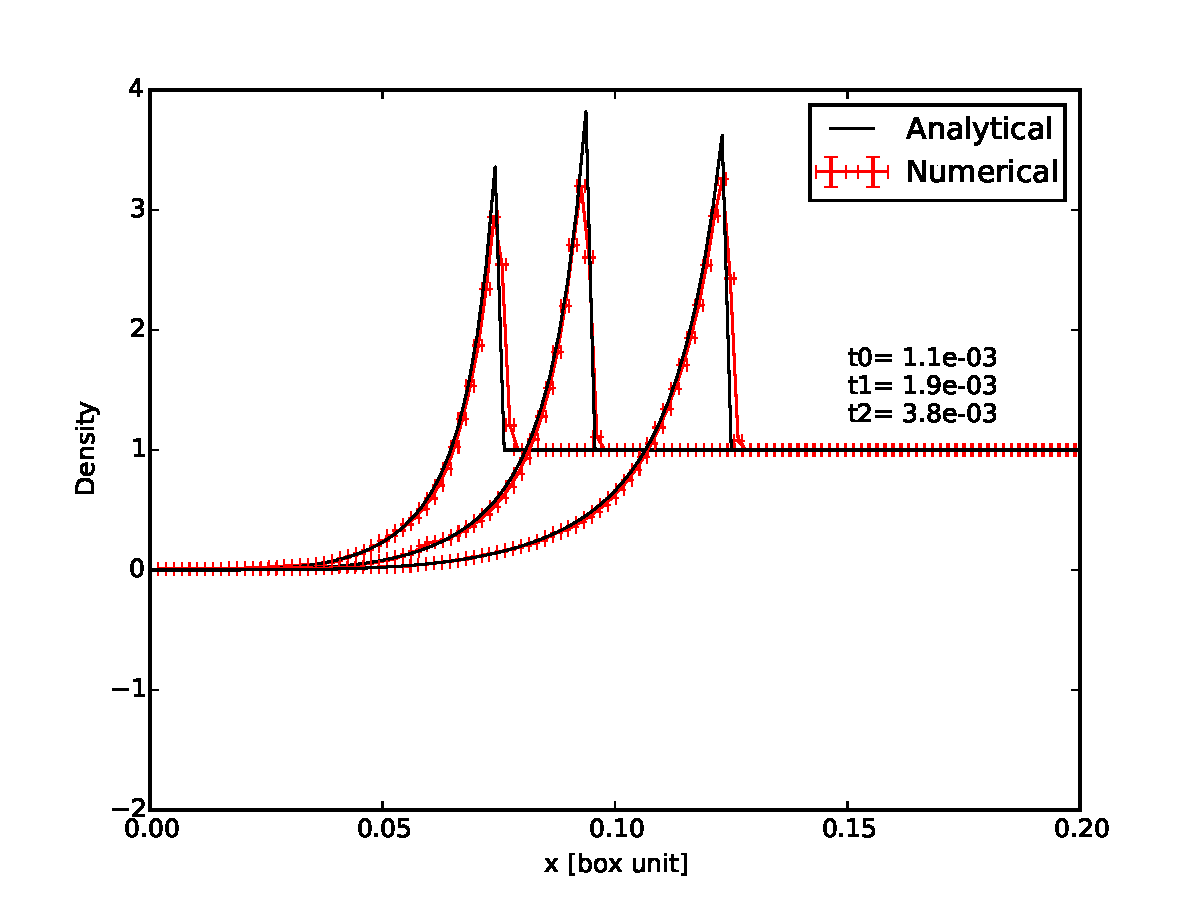
\includegraphics[height=.3\textheight]{img/03/sedov/sedov_evol_8_den_lin.pdf} 
		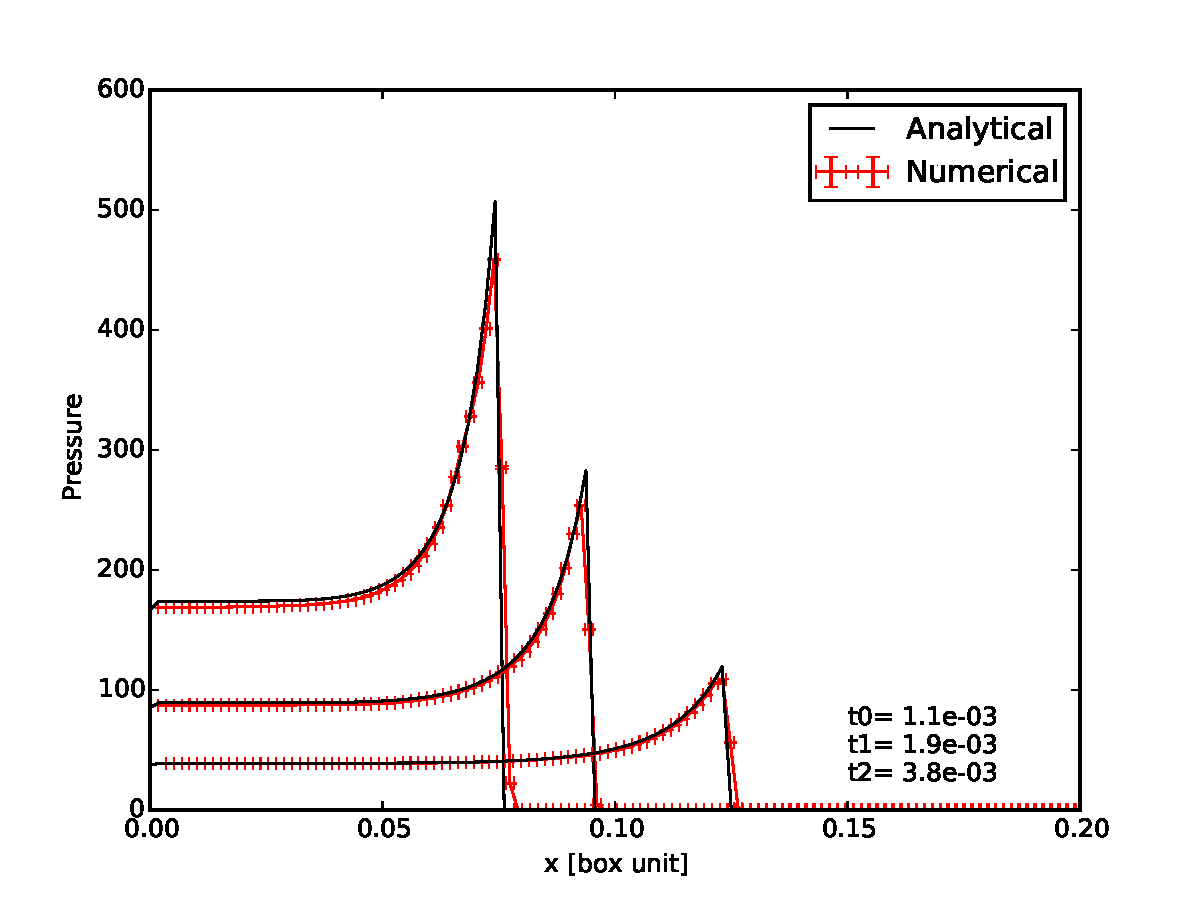
\includegraphics[height=.3\textheight]{img/03/sedov/sedov_evol_8_pres.pdf} 
		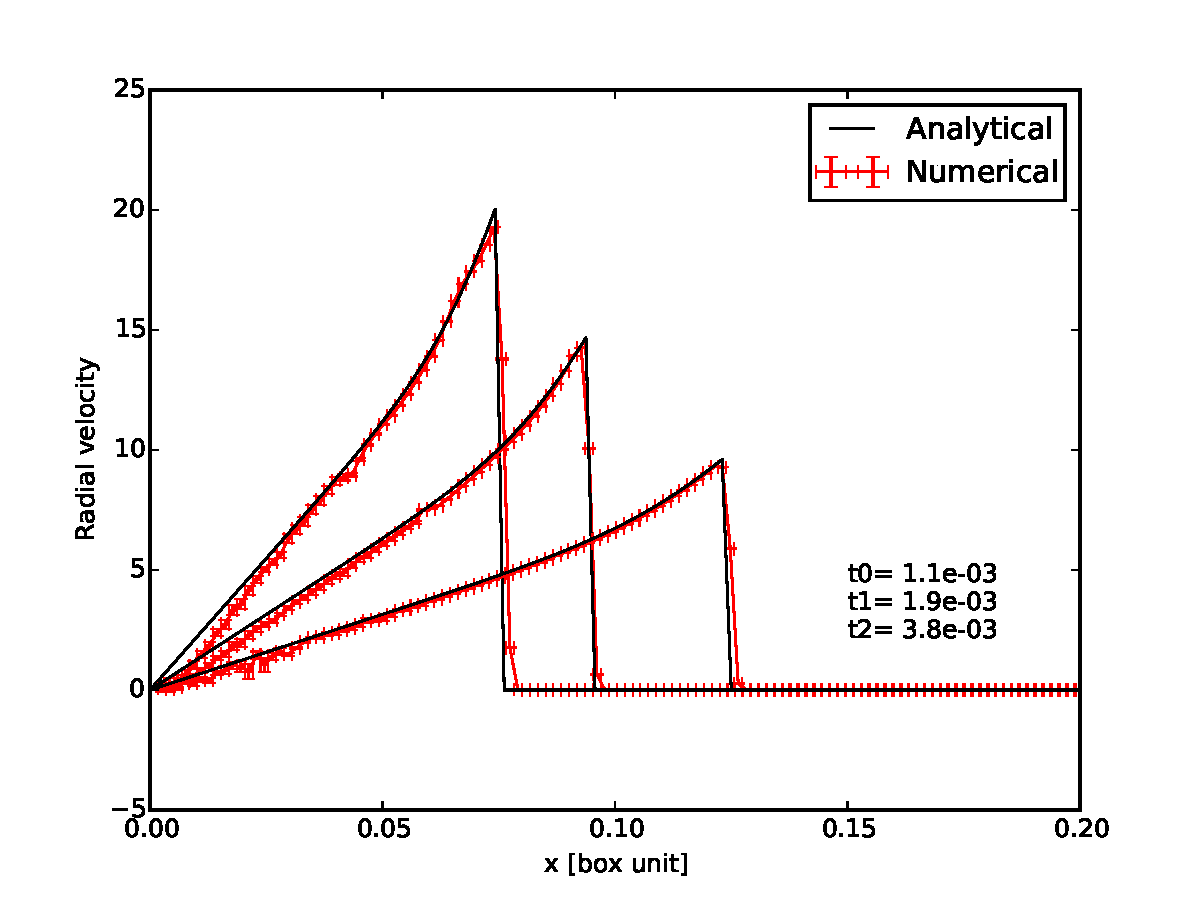
\includegraphics[height=.3\textheight]{img/03/sedov/sedov_evol_8_vel.pdf} 
        \caption{Test de Sedov, évolution des différentes variables d'états. La densité en haut, la pression au milieu et la vitesse radiale en bas.}
 		\label{fig:sedov_evol}
\end{figure}



\subsubsection{Sedov comparaison entre les méthodes}

Nous avons vu qu'il existe différents moyens d'injecter de l'énergie dans le solveur hydrodynamique.
Le test présenté ici consiste a vérifié que les différentes méthodes sont équivalentes entre elles.

Nous allons comparer 3 méthodes : 
\begin{itemize}
\item l'injection thermique dans une cellule 
\item l'injection thermique dans un cube de huit cellules
\item l'injection cinétique  dans un cube de huit cellules
\end{itemize}


Ces 3 tests utilisent cette fois ci espace discret de  $128^3$ éléments, mais en autorisant le raffinement sur 3 niveaux.
Le raffinement est effectué sur le gradient de densité, ie une cellule est divisé si le gradient de densité qu'elle contient est supérieur a une certaine valeur.
Cette méthode permet de concentrer le raffinement sur le front de l'onde choc.

La figure \ref{fig:sedovraff} présente le motif de raffinement obtenu pour le test d'injection thermique sur une cellule.
Tout les tests présentent un motif de raffinement similaire.

\begin{figure}[htpb]
        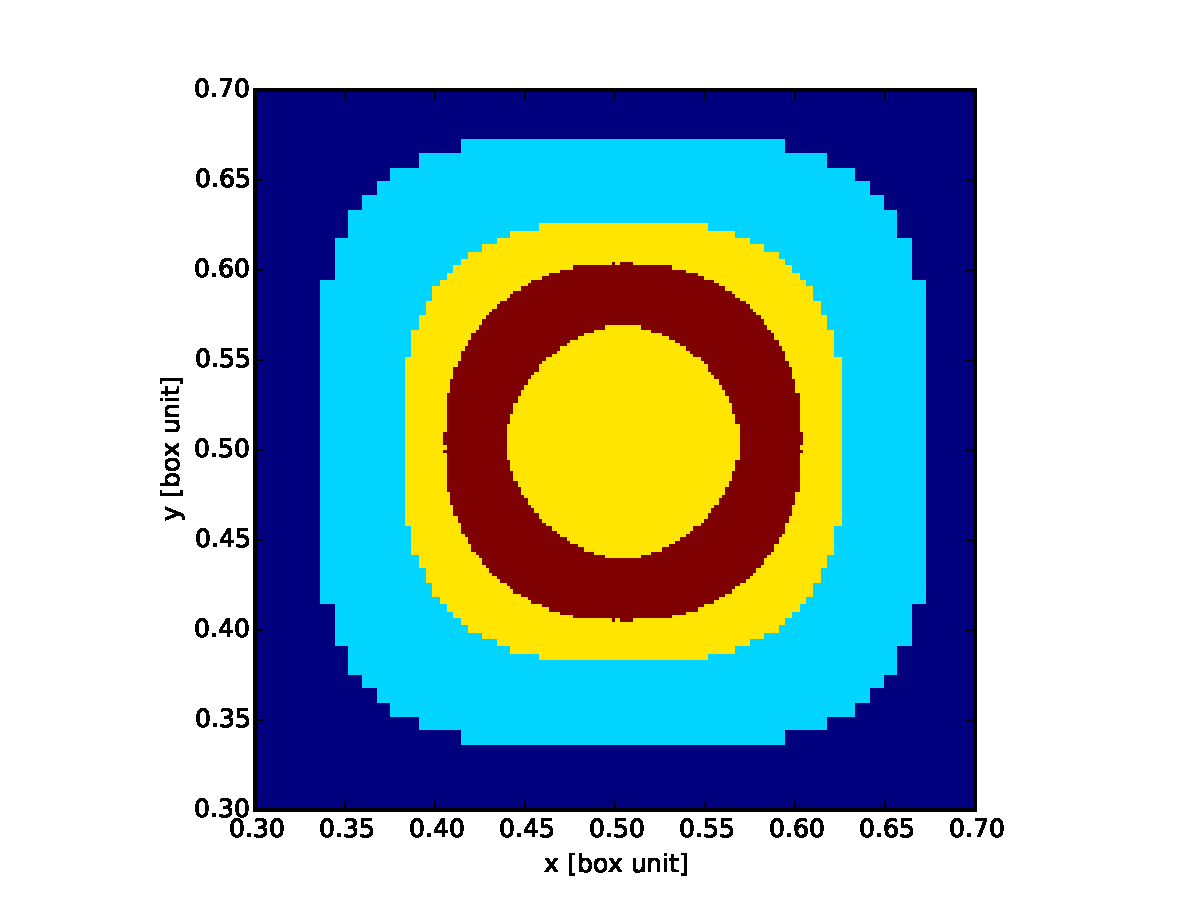
\includegraphics[width=.95\linewidth]{img/03/sedov/slice_th_1raf.pdf} 
        \caption{Test de Sedov, raffinement (mettre la color map) }
 		\label{fig:sedovraff}
\end{figure}

La figure \ref{fig:sedovmethod} presente les profils obtenus a un instant donné pour les différentes méthodes d'injection d'énergie et pour les différents champs.
On observe que le front est bien situé au même endroits indépendamment de la méthode.
%Le profil de densité est présenté en échelle logarithmique pour accentuer les difference au niveau du centre. 

\begin{figure}[htpb]
        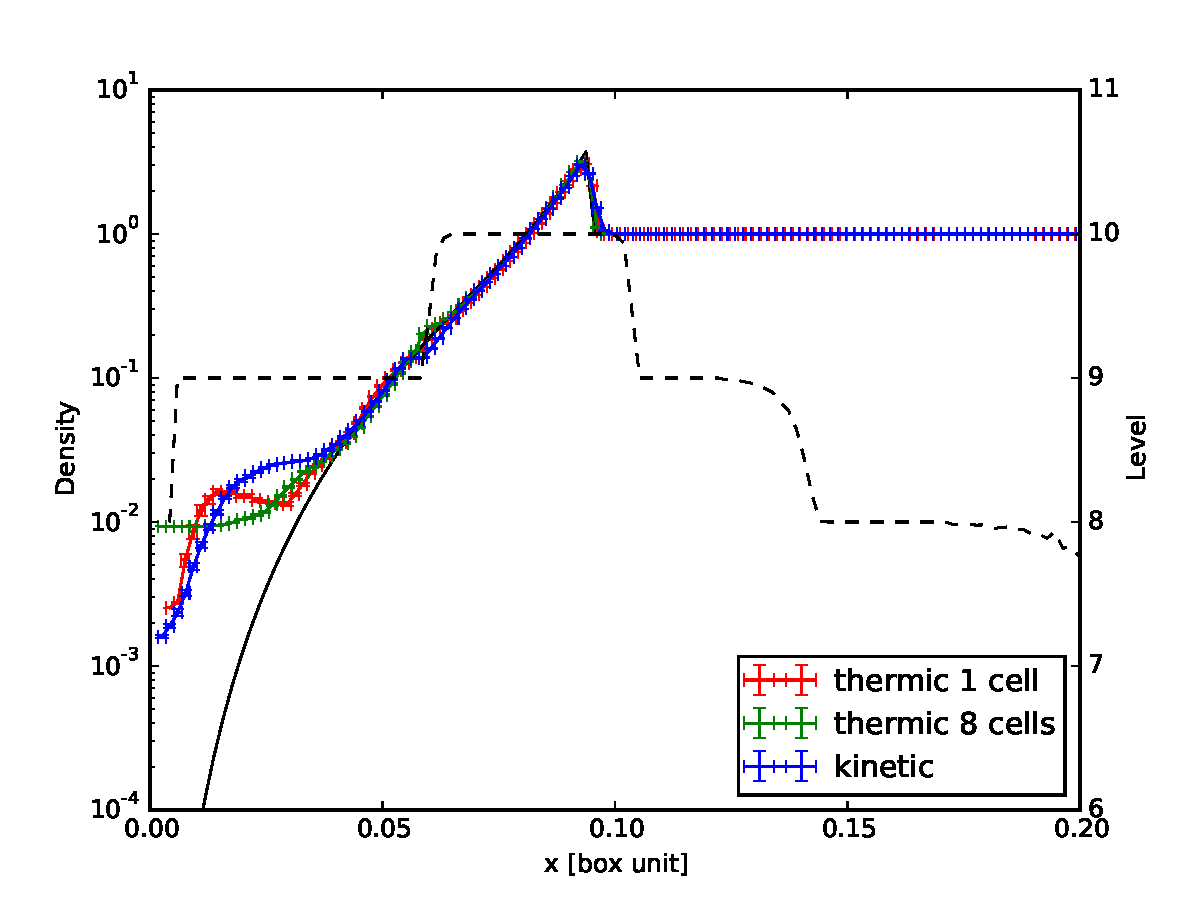
\includegraphics[height=.3\textheight]{img/03/sedov/sedov_comp_profile_den.pdf} 
		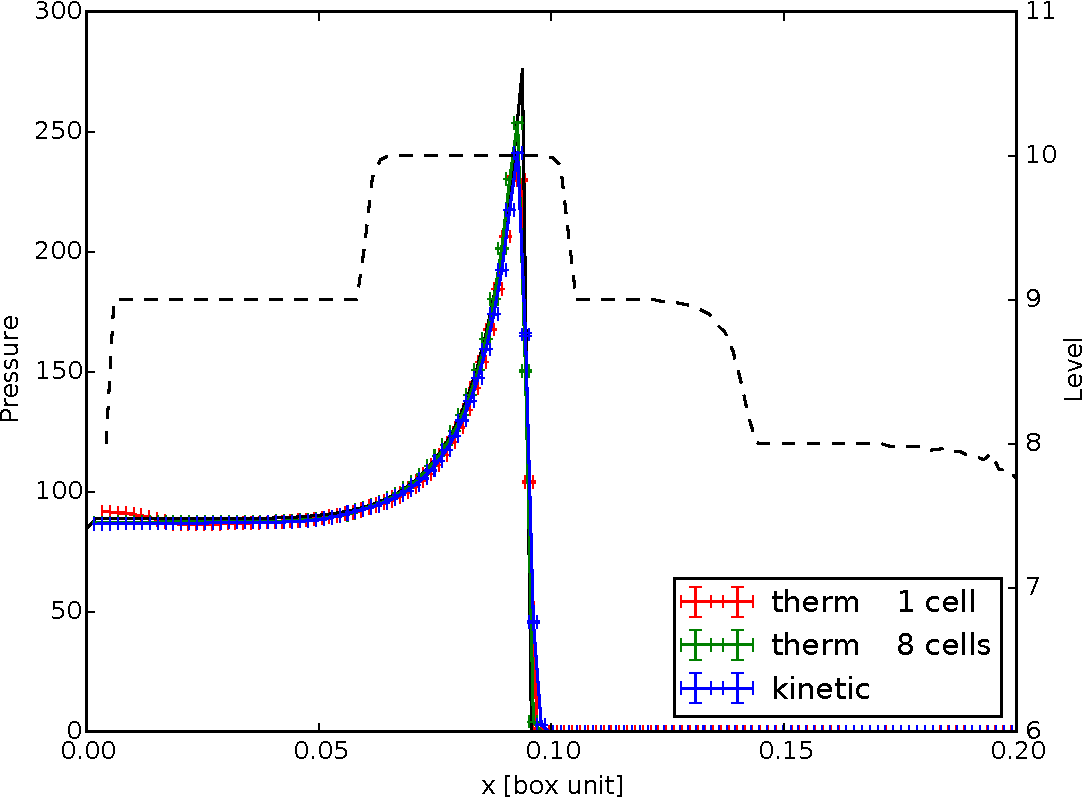
\includegraphics[height=.3\textheight]{img/03/sedov/sedov_comp_profile_pres.pdf} 
		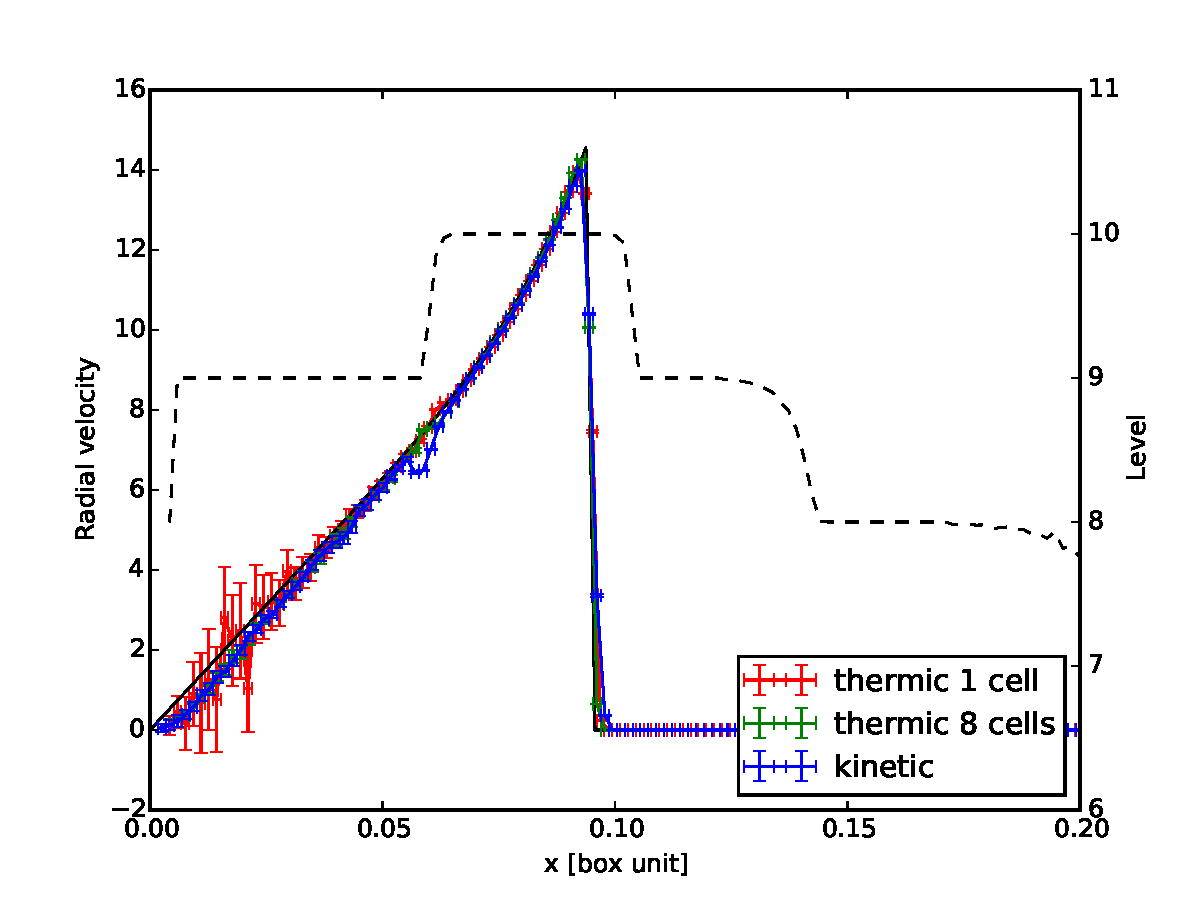
\includegraphics[height=.3\textheight]{img/03/sedov/sedov_comp_profile_vel.pdf} 
        \caption{Test de Sedov, comparaison des profil radial en fonction des  méthodes d'injection. 
        Densité en haut, pression au milieu et vitesse radial en bas.
        La position et la forme du front d'onde ne dépendent pas de la méthodes d'injection utilisée.}
 		\label{fig:sedovmethod} 
\end{figure}


Même si les profils radiaux moyens sont comparables, on observe des différences sur la forme de l'explosion.
La figure \ref{fig:sedovslice} présente une coupe suivant l'axe z de la grille, contenant la cellule d'injection, pour les trois méthodes.
Ces différence sont dues a la grille et a la façon dont les flux sont calculés.
Dans le cas de l'injection thermique, les flux auront tendance à être suivant les axes principaux de la grille.
Ce qui donne ce motif en forme de "+" bien particulier.
Dans le cas de l'injection cinétique, les sont forcés a être dans des directions obliques, a 45°, par rapport a la l'axe de la grille.
Nous avons cette fois si une figure en forme de "x".

\begin{figure}[htpb]
        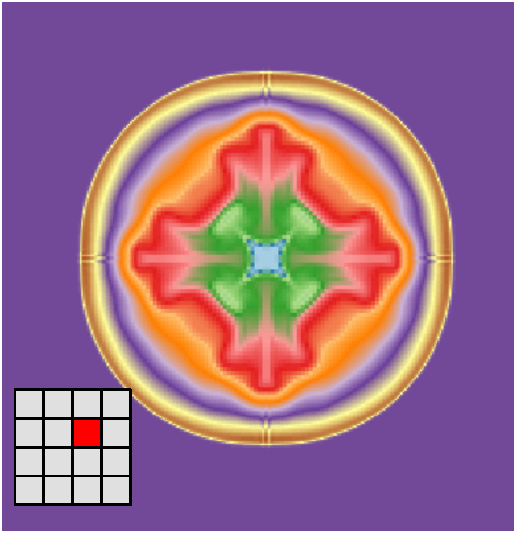
\includegraphics[height=.3\textheight]{img/03/sedov/slice_therm1.pdf} 
		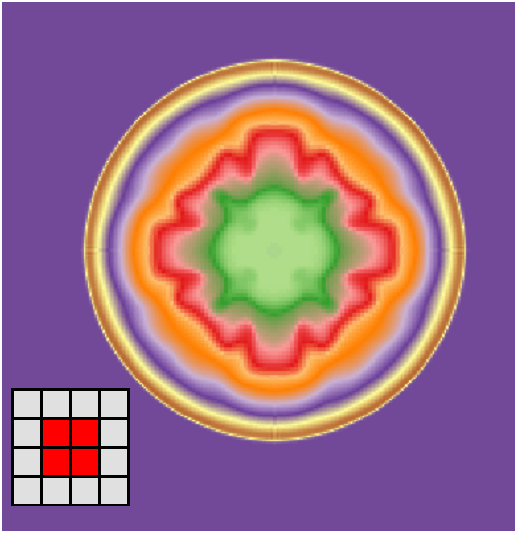
\includegraphics[height=.3\textheight]{img/03/sedov/slice_therm4.pdf} 
		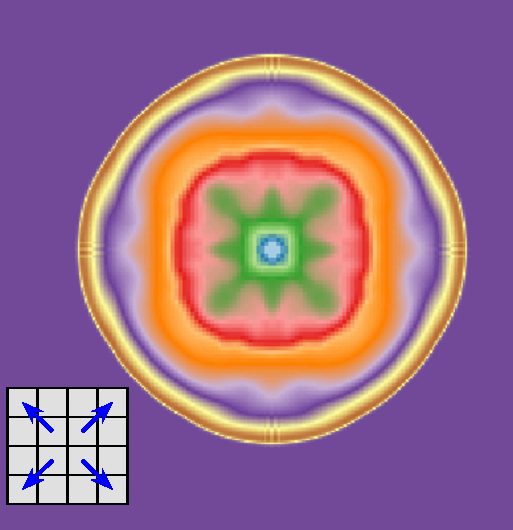
\includegraphics[height=.3\textheight]{img/03/sedov/slice_kin.pdf} 
        \caption{Test de Sedov}
 		\label{fig:sedovslice}
\end{figure}



\subsubsection{Conclusion}

La conclusion de ses tests est que les différentes méthodes d'injection sont équivalentes, au moins dans le contexte du test de Sedov.

%OK\\
%mais pas en cosmo




le pas de temps\\
\section{test}
fonction de luminosité 
